% --------------------------------------------------------------------------- %
% Poster about FURAX: A Novel Approach to Optimize Clustering of Parametric  %
% Map-Based Component Separation for Upcoming CMB Polarization Satellites     %
% --------------------------------------------------------------------------- %
% Created using Brian Amberg's LaTeX Poster Template                         %
% Content adapted from the FURAX component separation paper                  %
% --------------------------------------------------------------------------- %

\documentclass[a2paper,portrait,fontscale=0.9]{baposter}

\usepackage{relsize}		% For \smaller
\usepackage{url}			% For \url
\usepackage{graphicx} % Required for resizing symbols
\usepackage{enumitem} % Required for customizing lists
\usepackage{caption}
\usepackage{xcolor} % Required for colors
\usepackage{pifont}
\usepackage{amsmath}
\usepackage{amssymb}
\usepackage{natbib}
\usepackage{svg}
\usepackage{listings}
\usepackage{xcolor} % Make sure xcolor is loaded before listings for color definitions
% Using natbib instead of biblatex for better compatibility

% Define a custom style for Python code
\lstdefinestyle{custompy}{
    language=Python,
    basicstyle=\footnotesize\ttfamily, % Use a small, monospaced font
    keywordstyle=\color{blue}\bfseries,
    stringstyle=\color{purple},
    commentstyle=\color{gray},
    numbers=none,
    showstringspaces=false,
    breaklines=true, % Automatically break long lines
    frame=none, % No frame around the code
    backgroundcolor=\color{white}, % Set a background color if needed
    tabsize=2
}

\newlist{arrowlist}{itemize}{1}
\setlist[arrowlist]{label=$\resizebox{!}{5pt}{\textbullet}$}
\newcommand{\highlight}[1]{\textbf{\textcolor{red}{#1}}}

\definecolor{darkblue}{rgb}{0.0, 0.0, 0.5}
%%% Global Settings %%%%%%%%%%%%%%%%%%%%%%%%%%%%%%%%%%%%%%%%%%%%%%%%%%%%%%%%%%%

\graphicspath{{figures/}}	% Root directory of the pictures 

%%% Color Definitions %%%%%%%%%%%%%%%%%%%%%%%%%%%%%%%%%%%%%%%%%%%%%%%%%%%%%%%%%

\definecolor{bordercol}{RGB}{40,40,40}
\definecolor{headercol1}{RGB}{186,215,230}
\definecolor{headercol2}{RGB}{80,80,80}
\definecolor{headerfontcol}{RGB}{0,0,0}
\definecolor{boxcolor}{RGB}{240,240,255}
\definecolor{highlightbox}{RGB}{255,240,240}

%%%%%%%%%%%%%%%%%%%%%%%%%%%%%%%%%%%%%%%%%%%%%%%%%%%%%%%%%%%%%%%%%%%%%%%%%%%%%%%%
%%% Utility functions %%%%%%%%%%%%%%%%%%%%%%%%%%%%%%%%%%%%%%%%%%%%%%%%%%%%%%%%%%

%%% Save space in lists. Use this after the opening of the list %%%%%%%%%%%%%%%%
\newcommand{\compresslist}{
	\setlength{\itemsep}{1pt}
	\setlength{\parskip}{0pt}
	\setlength{\parsep}{0pt}
}

%%%%%%%%%%%%%%%%%%%%%%%%%%%%%%%%%%%%%%%%%%%%%%%%%%%%%%%%%%%%%%%%%%%%%%%%%%%%%%%
%%% Document Start %%%%%%%%%%%%%%%%%%%%%%%%%%%%%%%%%%%%%%%%%%%%%%%%%%%%%%%%%%%%
%%%%%%%%%%%%%%%%%%%%%%%%%%%%%%%%%%%%%%%%%%%%%%%%%%%%%%%%%%%%%%%%%%%%%%%%%%%%%%%

\begin{document}

\typeout{Poster rendering started}

%%% Setting Background Image %%%%%%%%%%%%%%%%%%%%%%%%%%%%%%%%%%%%%%%%%%%%%%%%%%
\background{
	\begin{tikzpicture}[remember picture,overlay]%
	\draw (current page.north west)+(-2em,2em) node[anchor=north west]
	{
\includegraphics[height=1.1\textheight]{pix/background}};
	\end{tikzpicture}
}

%%% General Poster Settings %%%%%%%%%%%%%%%%%%%%%%%%%%%%%%%%%%%%%%%%%%%%%%%%%%%
%%%%%% Eye Catcher, Title, Authors and University Images %%%%%%%%%%%%%%%%%%%%%%
\begin{poster}{
	grid=false,
	eyecatcher=true, 
	borderColor=bordercol,
	headerColorOne=headercol1,
	headerColorTwo=headercol2,
	headerFontColor=headerfontcol,
	boxColorOne=boxcolor,
	headershape=rounded,
	headerfont=\Large\sf\bf,
	textborder=roundedright,
	background=user,
	headerborder=open,
    columns=2,
    colspacing=2em,
  boxshade=plain
}
%%% Eye Cacther %%%%%%%%%%%%%%%%%%%%%%%%%%%%%%%%%%%%%%%%%%%%%%%%%%%%%%%%%%%%%%%
{
}
%%% Title %%%%%%%%%%%%%%%%%%%%%%%%%%%%%%%%%%%%%%%%%%%%%%%%%%%%%%%%%%%%%%%%%%%%%
{\sf\bf
    A Novel Approach to Optimize Clustering of Parametric Map-Based Component Separation for Upcoming CMB Polarization Satellites
}
%%% Authors %%%%%%%%%%%%%%%%%%%%%%%%%%%%%%%%%%%%%%%%%%%%%%%%%%%%%%%%%%%%%%%%%%%
{
    \vspace{1em} Wassim Kabalan$^{1}$, Wuhyun Sohn$^{1}$, Benjamin Beringue$^{1}$, Artem Basyrov$^{1}$, Pierre Chanial$^{1}$, Alexandre Boucaud$^{1}$, Josquin Errard$^{1}$\\
    \vspace{1em}
    {\footnotesize 
        $^{1}$Université Paris Cité, CNRS, Astroparticule et Cosmologie, F-75013 Paris, France
    }
}
%%% Logo %%%%%%%%%%%%%%%%%%%%%%%%%%%%%%%%%%%%%%%%%%%%%%%%%%%%%%%%%%%%%%%%%%%%%%
{
% The logos are compressed a bit into a simple box to make them smaller on the result
\setlength\fboxsep{0pt}
\setlength\fboxrule{0.5pt}
	\fbox{
	\begin{minipage}{17em}
		
\includegraphics[width=17em,height=12em]{figures/scipol.jpeg}
	\end{minipage}
	}
}

% =============================================================================
% LEFT COLUMN
% =============================================================================

\headerbox{\textbf{Tensor-to-Scalar Ratio \& Foreground Removal}}{name=motivation,column=0,row=0,boxColorOne=highlightbox}{
\vspace{0.05cm}

\begin{minipage}{0.45\textwidth}
\centering
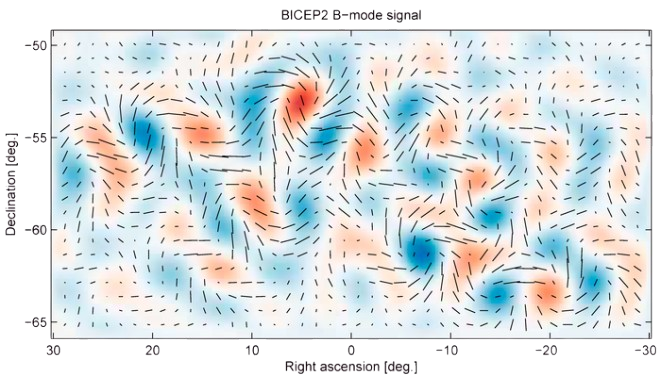
\includegraphics[width=\textwidth]{B-modes.png}
\captionof{figure}{CMB B-mode polarization signal from primordial gravitational waves}
\end{minipage}
\hfill
\begin{minipage}{0.45\textwidth}
\centering
\includesvg[width=\textwidth]{figures/foregrounds.svg}
\captionof{figure}{Galactic foreground contamination}
\end{minipage}

\vspace{0.05cm}

\textbf{The Challenge:}
\begin{itemize}[leftmargin=0.5cm] \compresslist
    \item[\ding{227}] Measuring tensor-to-scalar ratio $r$ requires detecting faint B-mode polarization
    \item[\ding{227}] Galactic foregrounds dominate CMB signal by orders of magnitude
    \item[\ding{227}] \highlight{Accurate foreground removal is critical for $r < 0.001$ detection}
\end{itemize}

\vspace{0.05cm}
}
\headerbox{\textbf{Parametric Component Separation}}{name=parametric,column=0,below=motivation}{
\vspace{0.05cm}

\textbf{The Standard Model:}
The observed sky signal ($\mathbf{d}$) in each pixel is modeled as a linear combination of astrophysical components ($\mathbf{s}$) and instrumental noise ($\mathbf{n}$).
\begin{equation}
    \mathbf{d} = \mathbf{A}(\boldsymbol{\beta})\,\mathbf{s} + \mathbf{n} \label{eq:model}
\end{equation}
The goal is to solve for the components $\mathbf{s}$, particularly the CMB, by estimating the spectral parameters $\boldsymbol{\beta}$ that define the mixing matrix $\mathbf{A}$.

\vspace{0.05cm}

\textbf{Spectral Likelihood:}
\begin{equation}
    \ln \mathcal{L}_{\mathrm{spec}}(\boldsymbol{\beta}) \propto (\mathbf{A}^\top \mathbf{N}^{-1} \mathbf{d})^\top (\mathbf{A}^\top \mathbf{N}^{-1} \mathbf{A})^{-1} (\mathbf{A}^\top \mathbf{N}^{-1} \mathbf{d})
\end{equation}
\citep{Stompor_2009}
\vspace{0.05cm}
}

\headerbox{\textbf{Modeling Spatially-Varying Foregrounds}}{name=spatial,column=0,below=parametric}{
\vspace{0.05cm}

\textbf{Foreground Spectral Parameters Vary Across Sky:}

\begin{center}
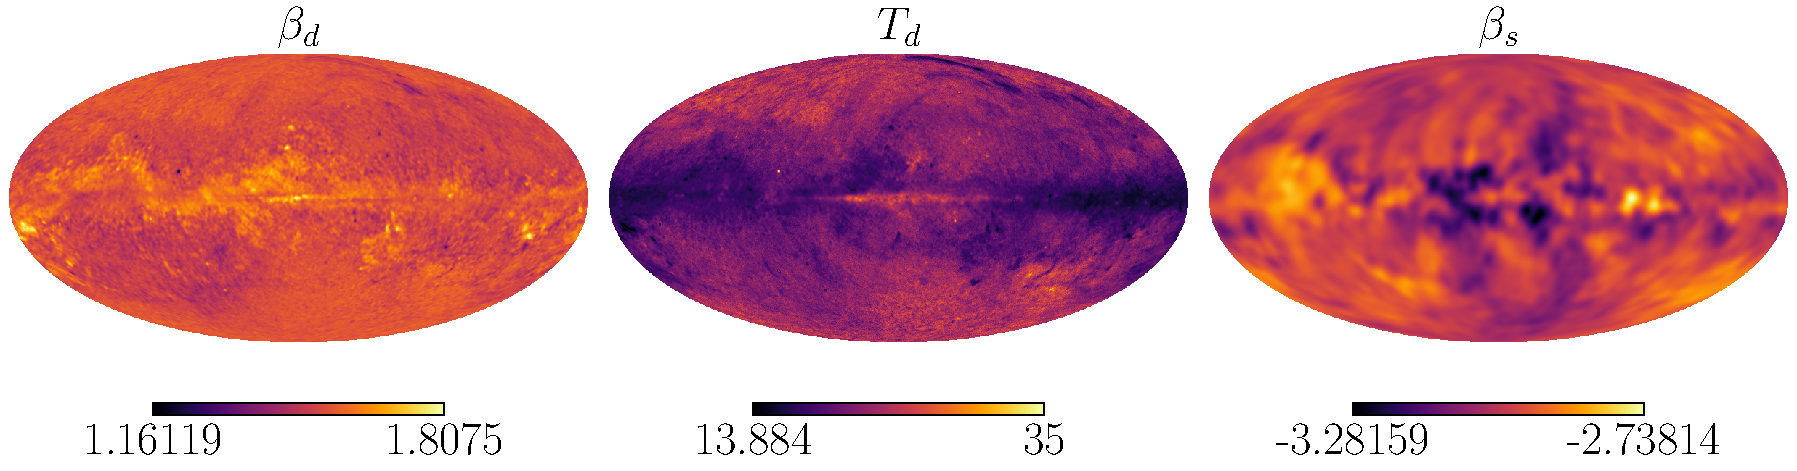
\includegraphics[width=0.60\textwidth]{mbb_index_map.pdf}
\captionof{figure}{Modifid blackbody spectral index map showing spatial variability in dust emission properties across the sky}
\end{center}

\textbf{Clustering Approach:}
\begin{itemize}[leftmargin=0.5cm] \compresslist
    \item[\ding{227}] Spherical K-means clustering groups pixels with similar spectral properties
    \item[\ding{227}] Balances statistical uncertainty with modeling flexibility
\end{itemize}

\vspace{0.05cm}

\textbf{Optimized K-means Parameters:}
\begin{center}
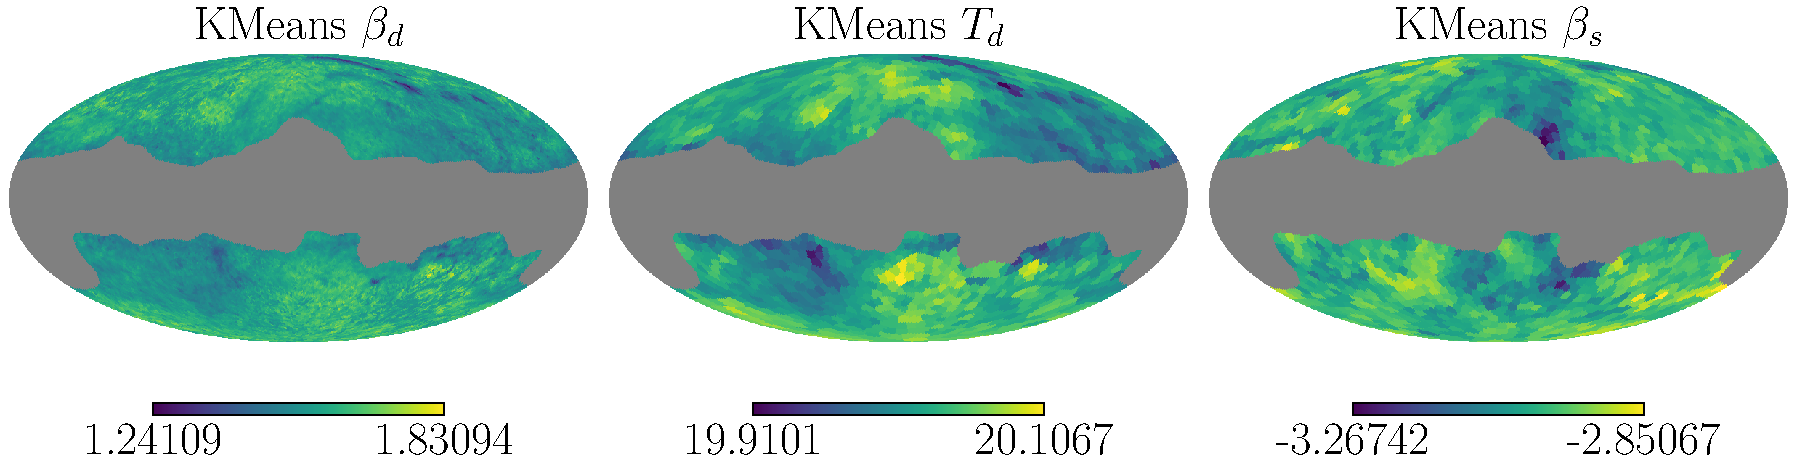
\includegraphics[width=0.60\textwidth]{params_KMeans.pdf}
\captionof{figure}{Optimized spectral parameter distributions from K-means clustering showing data-driven adaptation to foreground complexity}
\end{center}

\vspace{0.05cm}
}


% =============================================================================
% RIGHT COLUMN
% =============================================================================


\headerbox{\textbf{The FURAX Framework: A Scalable JAX-Native Engine}}{name=furax,column=1,row=0,span=1}{
\vspace{0.05cm}

% Use minipages to organize content
\begin{minipage}{0.52\textwidth}
    \textbf{Core Features:}
    \begin{itemize}[leftmargin=0.5cm] \compresslist
        \item[\ding{227}] \textbf{JAX-Native}: End-to-end differentiable \& GPU accelerated. \citep{FURAX}
        \item[\ding{227}] \textbf{Modular Design}: Composable algebraic operators for complex models.
        \item[\ding{227}] \textbf{Memory Efficient}: Matrix-free operators enable high-resolution analysis.
        \item[\ding{227}] \textbf{Scalable}: Distributed parallelism for HPC clusters.
    \end{itemize}
    
    \vspace{0.05cm}
    
    \textbf{Elegant Implementation:}
    \centering
    \fbox{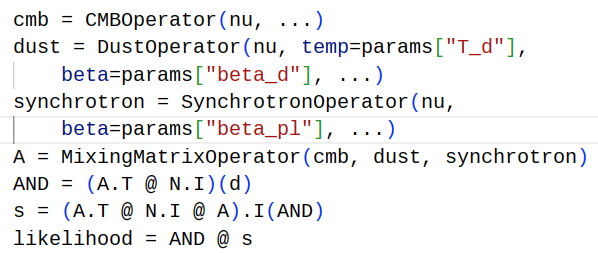
\includegraphics[width=0.9\linewidth]{figures/snippet.png}}
    
\end{minipage}
\hfill % Spacer
\begin{minipage}{0.45\textwidth}
    \textbf{Unprecedented Speed:}
    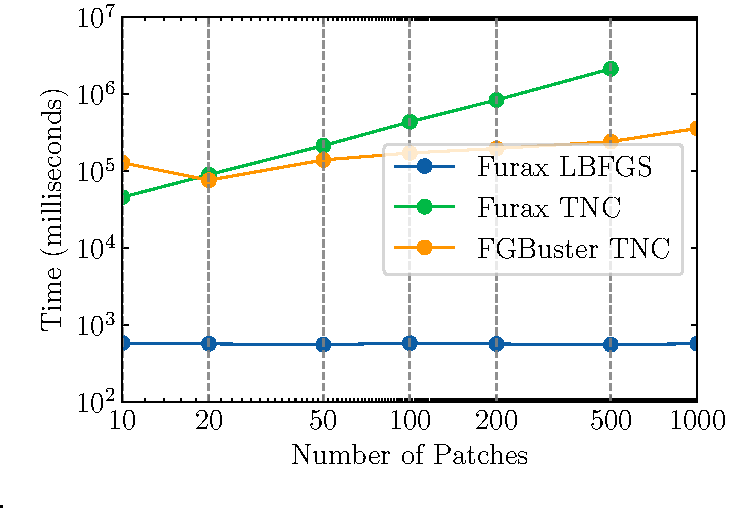
\includegraphics[width=\linewidth]{figures/runtime_comparison.pdf}
    \captionof{figure}{\textit{FURAX (LBFGS) scales robustly with the number of patches, consistently outperforming older frameworks like FGBuster.}}
\end{minipage}

\vspace{0.05cm}

\textbf{Enabling a Grid Search at Scale:} The performance of FURAX allowed us to run $\sim$1.92 million independent component separation fits to find the optimal clustering configuration, a task infeasible with previous tools.
} 



\headerbox{\textbf{Selection Criterion: Minimizing CMB Variance}}{name=analysis,column=1,below=furax}{
\vspace{0.03cm}

\textbf{Selection Criterion - CMB Variance Minimization:}
\begin{equation}
    \sigma^2_{\mathrm{CMB}} = \left\langle \mathrm{Var}_{i} \left[ \hat{s}^{(i)}_{\mathrm{CMB}} \right] \right\rangle_{\text{pixels}}
\end{equation}

\begin{center}
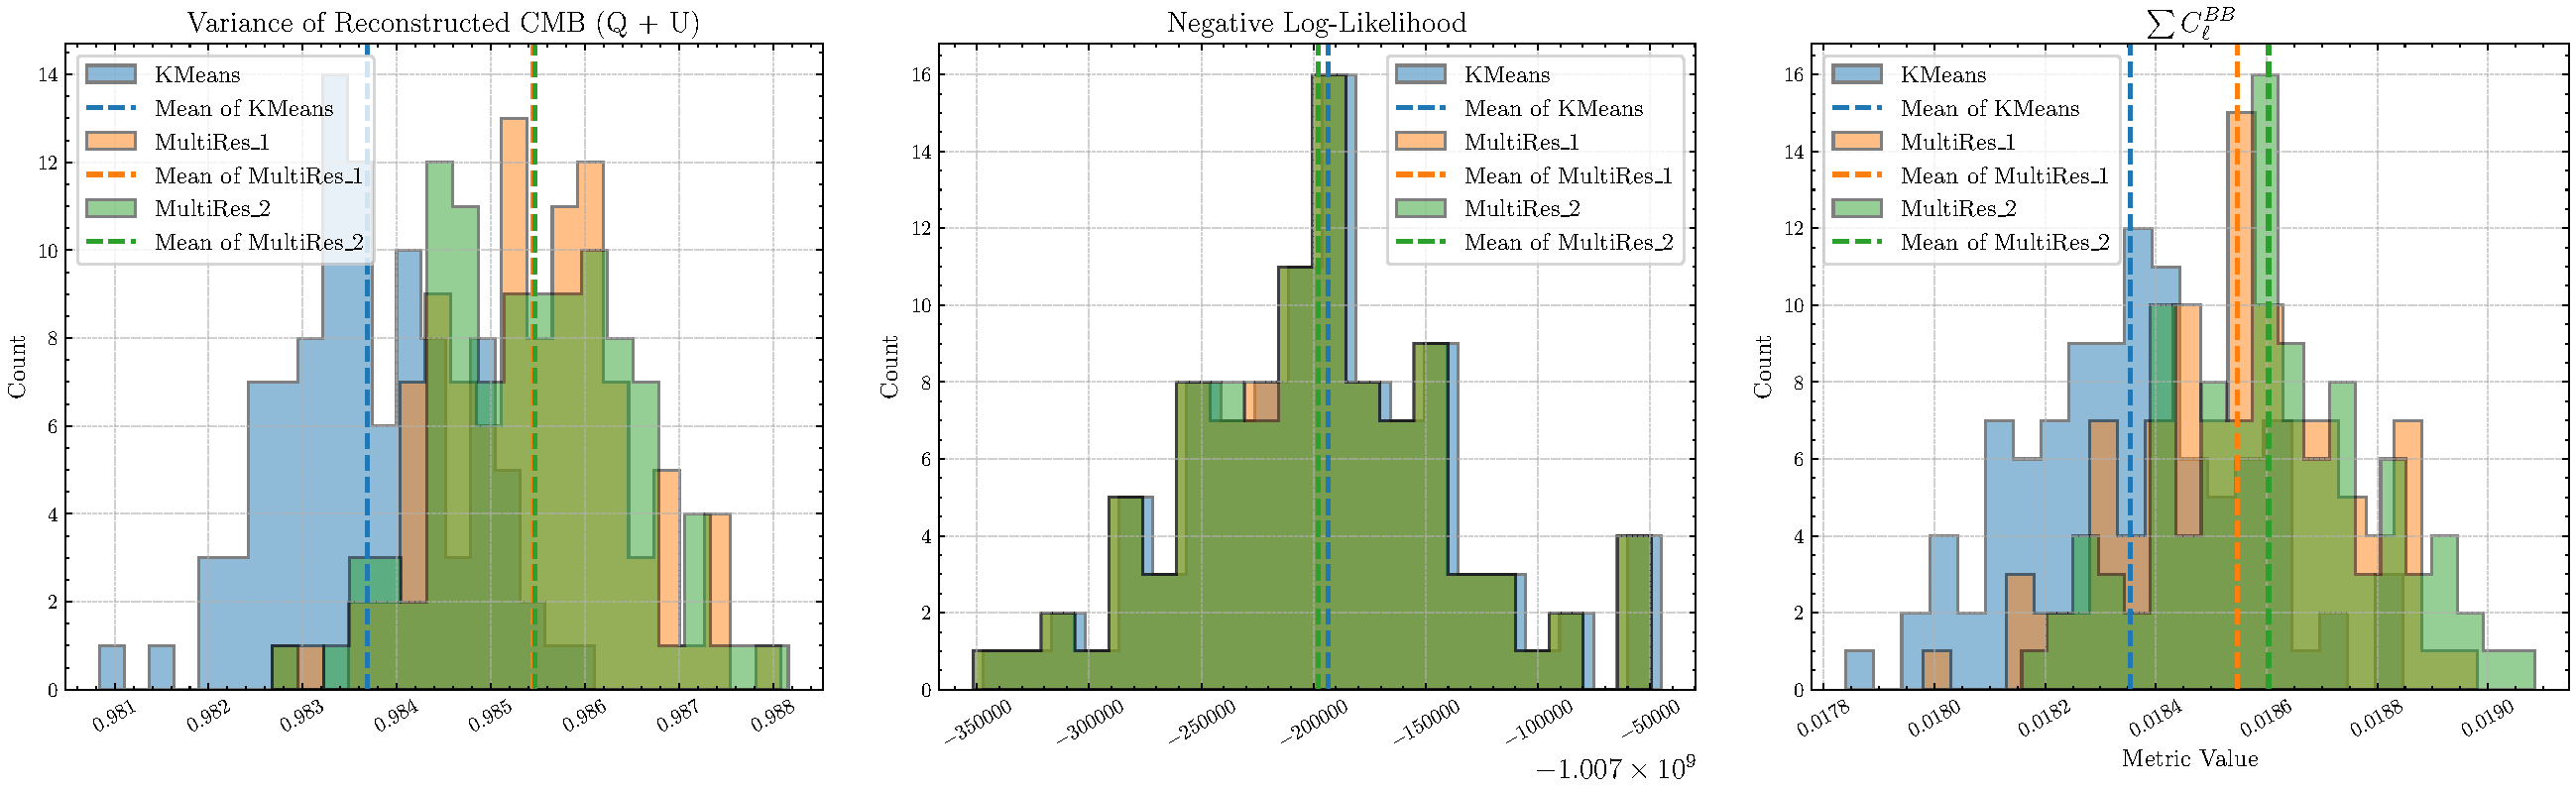
\includegraphics[width=1.0\textwidth]{variance_likelihood_distributions.pdf}
\captionof{figure}{Distribution of CMB variance, spectral likelihood, and B-mode power for different spatial modeling approaches. K-means clustering achieves optimal balance.}
\end{center}

\textbf{Key Insight:} Variance minimization acts as proxy for residual foreground contamination, leading to more robust cosmological constraints.

\vspace{0.15cm}
}

\headerbox{\textbf{Comparing Clustering Strategies: Data-Driven vs. Fixed-Resolution}}{name=patches,column=1,below=analysis}{
\vspace{0.05cm}

% Use two minipages for a side-by-side comparison.
\begin{minipage}{0.50\textwidth}
    \centering
    \textbf{K-means Clustering (Our Method)}
    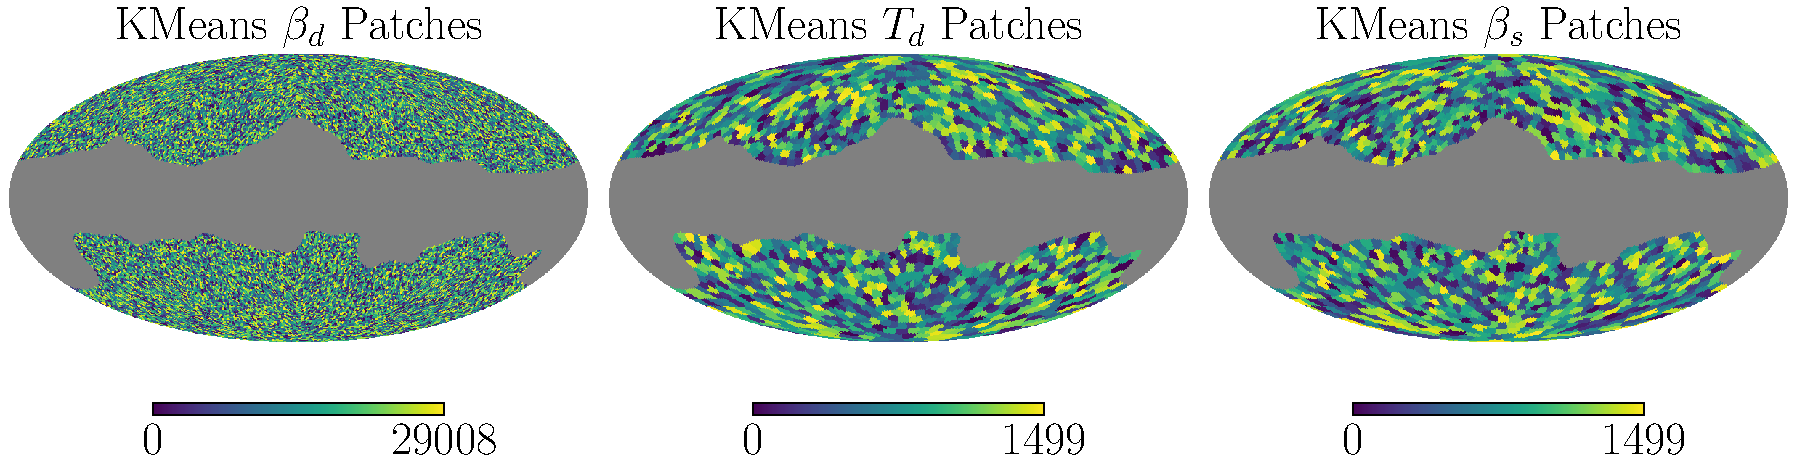
\includegraphics[width=\linewidth]{figures/patches_KMeans.pdf}
    \captionof{figure}{\textit{Flexible, data-driven patches adapt to foreground complexity by minimizing CMB variance. This corresponds to Figure 7 in the paper.} \citep{JAXHEALPY}}
    \begin{itemize}[leftmargin=0.5cm] \compresslist
        \item[\ding{227}] Generates irregular, equal-area patches.
        \item[\ding{227}] Patch structure is learned from the data itself.
    \end{itemize}
\end{minipage}
\hfill % This creates space between the two minipages
\begin{minipage}{0.50\textwidth}
    \centering
    \textbf{Multi-Resolution (Baseline)}
    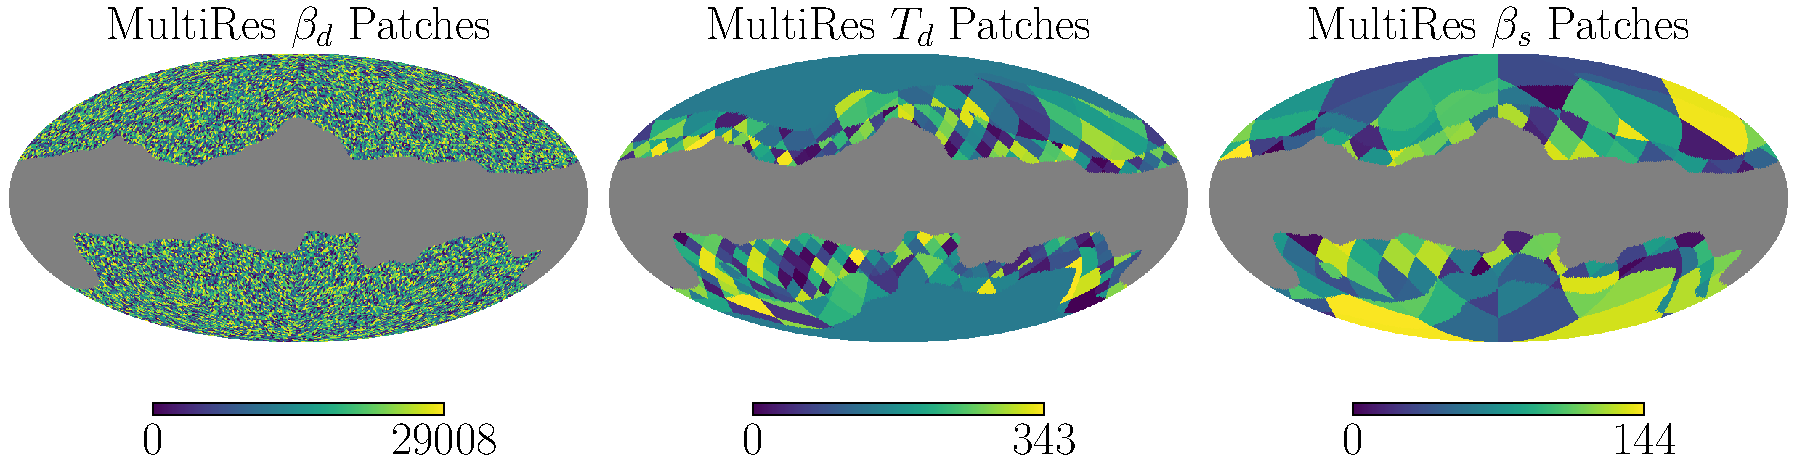
\includegraphics[width=\linewidth]{figures/patches_MultiRes.pdf}
    \captionof{figure}{\textit{Fixed, regular patches based on HEALPix downgrading, independent of sky variations. This corresponds to Figure 8 in the paper.} \citep{LiteBIRD_PTEP_2022}}
     \begin{itemize}[leftmargin=0.5cm] \compresslist
        \item[\ding{227}] Imposes a rigid, uniform grid.
        \item[\ding{227}] Lacks flexibility for complex regions.
    \end{itemize}
\end{minipage}

\vspace{0.15cm}
}

\headerbox{\textbf{Results}}{name=results,column=0,below=spatial,span=2}{
\vspace{0.05cm}
\begin{minipage}{0.48\textwidth}
    \textbf{Tensor-to-Scalar Ratio Constraints:}
    \begin{center}
        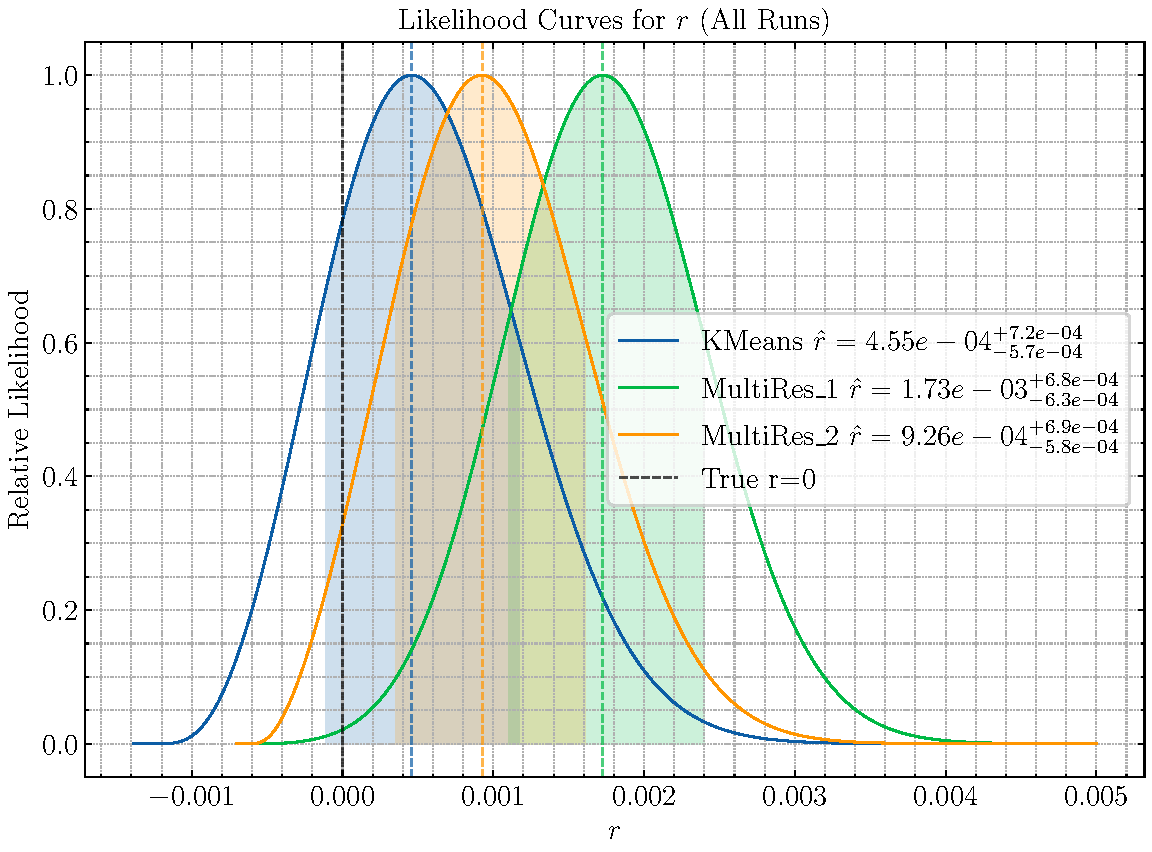
\includegraphics[width=0.75\textwidth]{r_likelihood_distribution.pdf}
        \captionof{figure}{$r$ likelihood distributions: K-means clustering (blue) yields $\hat{r} = 4.55 \times 10^{-4}$ with lowest bias and tightest constraints compared to multi-resolution approaches}
    \end{center}
\end{minipage}
\hfill
\begin{minipage}{0.48\textwidth}
    \textbf{Residual B-mode Spectra:}
    \begin{center}
        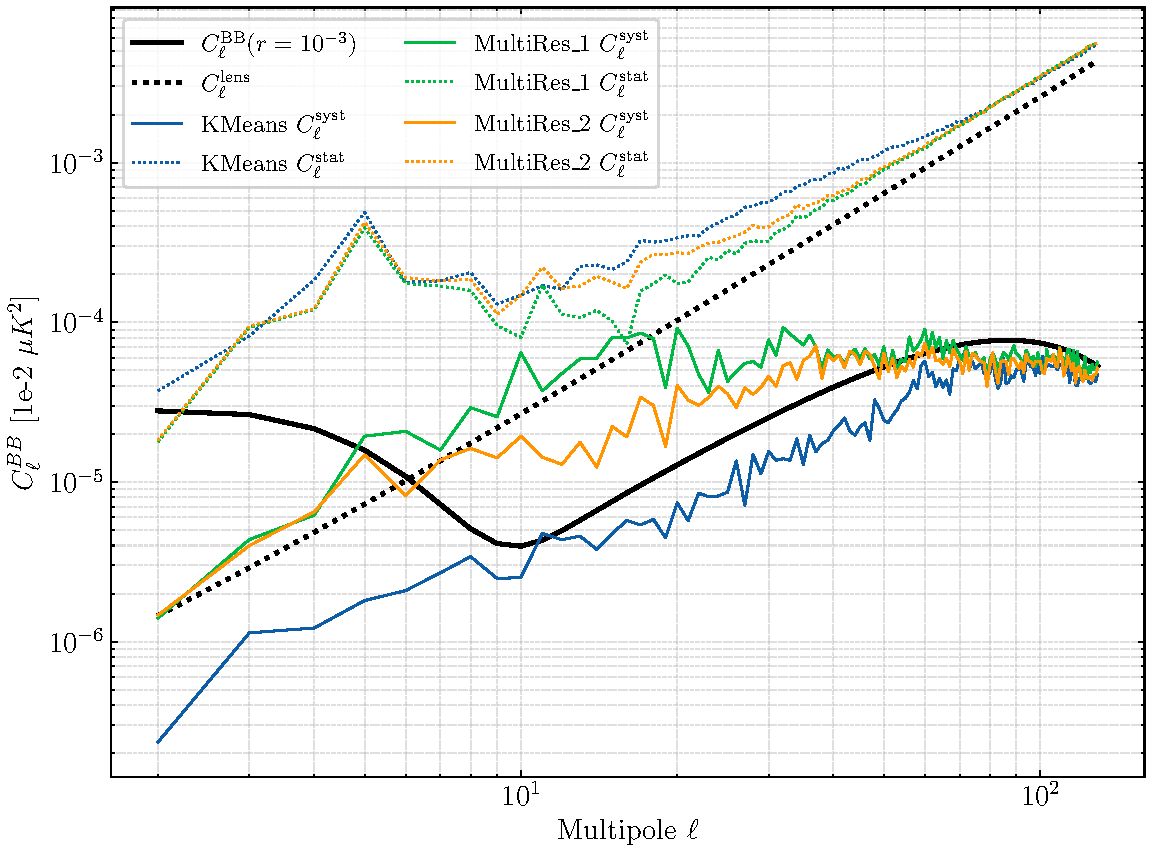
\includegraphics[width=0.75\textwidth]{bb_residual_spectra.pdf}
        \captionof{figure}{Residual B-mode power spectra: K-means clustering (blue) achieves significantly lower systematic residuals compared to multi-resolution approaches, falling below target sensitivity levels}
    \end{center}
\end{minipage}
    
\vspace{0.01cm}
}

% =============================================================================
% BOTTOM SECTION - REFERENCES
% =============================================================================

\headerbox{\textbf{References \& Acknowledgements}}{name=references,column=0,below=results,span=2}{
\vspace{0.01cm}

% Make bibliography compact
\setlength{\bibsep}{0pt}
\small
\setlength{\itemsep}{0pt}
\setlength{\parsep}{0pt}
\bibliography{biblio}
\bibliographystyle{unsrt}

\textbf{Acknowledgements:} This work was supported by the \textsc{SciPol} project (ERC Grant No. 101044073, PI: Josquin Errard) and performed using HPC resources at IDRIS Jean Zay supercomputer. Full code available at: \url{https://github.com/ASKabalan/furax-compsep-paper}

\vspace{0.01cm}
}

\end{poster}
\end{document}